\begin{figure}[!htb]\centering
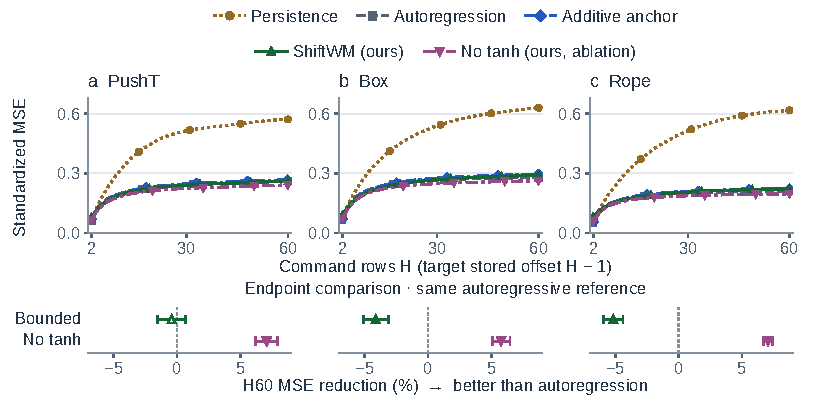
\includegraphics[width=\linewidth]{generated/iws_compact_evidence/forecast_and_gain.pdf}
\caption[Single-observation forecasts and paired gains.]{\textbf{Single-observation transfer: forecasting and the effect of the correction bound.} Top: all five predictors and all 59 future offsets on recorded IWS tasks; $H$ counts native command rows and predicts stored offset $H-1$. Bottom: $H=60$ MSE reduction versus the same autoregressive baseline; right is better and bars are paired 95\% intervals. The bounded model has no consistent advantage here; removing only $\tanh$ improves all three endpoint means. Means weight trajectories and three seeds equally. The original 27-model study and nine-model follow-up are development comparisons; the latter is exploratory. Table~\ref{tab:iws-development-complete} gives every plotted contrast and the original primary comparison; Table~\ref{tab:current-iws-scorecard} retains all four metrics. Reserved evaluation is excluded.}
\label{fig:iws-forecast-transfer}
\end{figure}
